\documentclass[11pt,a4paper]{article}
\usepackage[T1]{fontenc}
\usepackage[utf8]{inputenc}
\usepackage{lmodern}
\usepackage[a4paper,margin=25mm,headheight=15pt]{geometry}
\usepackage{microtype}
\usepackage{amsmath,amssymb,amsthm,mathtools}
\usepackage{booktabs,tabularx,longtable,array}
\usepackage{enumitem}
\usepackage{xcolor}
\usepackage{listings}
\usepackage{tikz}
\usetikzlibrary{arrows.meta,positioning,shapes.geometric,fit}
\usepackage[most]{tcolorbox}
\usepackage{fancyhdr}
\usepackage{xurl}
\usepackage[colorlinks=true,linkcolor=blue!45!black,citecolor=blue!45!black,urlcolor=blue!45!black]{hyperref}
\usepackage{bookmark}
\definecolor{ink}{HTML}{17324D}
\definecolor{soft}{HTML}{F3F6F9}
\definecolor{rulegray}{HTML}{CDD6DF}
\hypersetup{pdftitle={Motive: Concise Mathematical Reasoning with Kernel-Checked Elaboration},pdfauthor={OpenAI},pdfsubject={A proof-language design study grounded in ProveIt and Leant},pdfkeywords={Lean, proof language, proof synthesis, declarative proofs, formal verification}}
\pagestyle{fancy}
\fancyhf{}
\fancyhead[L]{\small\sffamily\color{ink}MOTIVE}
\fancyhead[R]{\small\sffamily A proof-language design study}
\fancyfoot[C]{\small\thepage}
\renewcommand{\headrulewidth}{0.3pt}
\setlength{\parskip}{4pt}
\setlength{\parindent}{1.2em}
\setcounter{tocdepth}{1}
\setlist{nosep,leftmargin=1.8em}
\emergencystretch=2em
\lstdefinestyle{proofcode}{basicstyle=\ttfamily\footnotesize,columns=fullflexible,keepspaces=true,breaklines=true,breakatwhitespace=false,showstringspaces=false,upquote=true,frame=single,rulecolor=\color{rulegray},backgroundcolor=\color{soft},framesep=7pt,xleftmargin=8pt,xrightmargin=8pt,aboveskip=10pt,belowskip=9pt,tabsize=2,escapeinside={(*@}{@*)}}
\lstset{style=proofcode}
\newtcolorbox{designbox}[1][]{colback=soft,colframe=rulegray,boxrule=0.5pt,arc=1pt,left=10pt,right=10pt,top=8pt,bottom=8pt,breakable,#1}
\newcommand{\Motive}{\textnormal{\textsc{Motive}}}
\newcommand{\code}[1]{\texttt{\detokenize{#1}}}
\newcommand{\N}{\mathbb N}
\newcommand{\Z}{\mathbb Z}
\newcommand{\R}{\mathbb R}
\newcommand{\E}{\mathcal E}
\newcommand{\Ob}{\mathcal O}
\newcommand{\ind}[1]{\mathbf 1_{\{#1\}}}
\newcommand{\Pcommit}{\texttt{24ce8bd743eaab64a91ce90725ea00f498d319d2}}
\newcommand{\Lcommit}{\texttt{c36adf114035fb2fba6c276b63944cc613b31668}}
\newcommand{\pfile}[1]{\href{https://github.com/VladimirReshetnikov/ProveIt/blob/24ce8bd743eaab64a91ce90725ea00f498d319d2/Analysis/FabiusFunction/Lean/FabiusFunction/#1}{\nolinkurl{#1}}}
\newcommand{\lfile}[1]{\href{https://github.com/VladimirReshetnikov/Leant/blob/c36adf114035fb2fba6c276b63944cc613b31668/#1}{\nolinkurl{#1}}}
\newtheorem{proposition}{Proposition}[section]
\newtheorem{definition}[proposition]{Definition}
\theoremstyle{remark}
\newtheorem{remark}[proposition]{Remark}
\newcolumntype{Y}{>{\raggedright\arraybackslash}X}
\begin{document}
\begin{titlepage}
\thispagestyle{empty}
\vspace*{12mm}
{\sffamily\large\color{ink}LANGUAGE DESIGN\quad /\quad FORMAL MATHEMATICS\par}
\vspace{12mm}
{\Huge\bfseries\color{ink}Motive\par}
\vspace{5mm}
{\LARGE\bfseries Concise Mathematical Reasoning\par}
\vspace{2mm}
{\LARGE\bfseries with Kernel-Checked Elaboration\par}
\vspace{9mm}
{\large A design study grounded in ProveIt and Leant\par}
\vspace{5mm}
{\normalsize Prepared for Vladimir Reshetnikov\par September 5, 2026\par}
\vspace{12mm}
\begin{abstract}
A mathematician may regard a proof as a substitution, a familiar identity, and a change of summation order. A formal development must also identify the precise types, justify the change of index, transport equalities, and discharge every side condition. The right response is not to discard these obligations, but to change who writes them. This article proposes \Motive, a provisional design for a mathematical proof language in which authors supply the structural decisions and the system reconstructs bounded, locally specified details. Its central object is a \emph{proof move with a contract}: a mathematical action accompanied by an exact input context, explicit output, generated obligations, and a kernel-checkable assembly procedure.

The proposal is grounded in three ProveIt developments---binomial inversion, elementary Lambert $W$ bounds, and geometric Richardson polynomials---and in Leant's separation of synthesis, candidate identity, and verification. Worked examples show what can safely become implicit and what must remain visible. The article gives an operational architecture, core elaboration rules, a relative soundness argument, a skeptical treatment of search failure, and a design for replayable proof artifacts. It also addresses statement fidelity, scope, classical assumptions, explanatory provenance, and fair evaluation. The proposed implementation is a layer over Lean rather than a replacement for its logic or mathematical library.
\end{abstract}
\vfill
\begin{designbox}
\textbf{Status.} This is a researched design proposal, not an implemented language. All \Motive\ listings are illustrative syntax. Repository observations come from pinned source inspection; the repositories were not rebuilt for this article. No compilation, proof-search success rate, or compression benchmark is claimed for the proposed language.
\end{designbox}
\end{titlepage}
\tableofcontents
\newpage

\section{The objective: shorter authorship, not weaker proof}
\label{sec:objective}
The most useful proof language would allow a mathematician to say what makes an argument work without continually describing how the underlying library represents it. This is a more demanding objective than reducing the number of characters. A proof consisting of a single opaque automation command can be short while communicating almost nothing. Conversely, a three-line calculation may contain more useful mathematical information than a compressed tactic expression that proves the same proposition.

The proposed division of labor is therefore:
\begin{quote}
The author specifies the mathematical landmarks and the reasons connecting them. The system reconstructs the representation changes and routine deductions, and supplies a checkable certificate for every omitted step.
\end{quote}
Here a \emph{landmark} is an intermediate assertion worth remembering: a useful substitution, a factorization, a reduction to a known theorem, or the invariant of an induction. A \emph{routine deduction} is not whatever a language model considers obvious. It is an obligation assigned to a declared reconstruction procedure with a specified theory, budget, and success criterion.

This design does not begin from the assumption that Lean lacks abstraction. Lean already separates a flexible surface language from its core, and supports extensible elaboration and proof automation. Its implicit arguments and existing proof constructs already perform substantial reconstruction \cite{lean4,lean-elab}. The repository examples also contain good abstractions and very short proofs. The question is where another abstraction layer would make \emph{authorship and explanation} better, not whether verbose source should simply be replaced by stronger automation.

\subsection{Three kinds of detail}
A useful distinction is between \emph{mathematical decisions}, \emph{representation obligations}, and \emph{interaction overhead}. Choosing the substitution $k=j+i$ is a mathematical decision. Showing that it bijects two specified finite intervals is an obligation induced by that decision. Selecting the exact library lemma spelling and supplying its arguments in the expected order is often interaction overhead.

These categories are contextual. In a first proof of a change-of-variables theorem, the bijection may be the central mathematical content. In an application of that theorem, its interval arithmetic may be routine. Accordingly, \Motive\ should not permanently label whole classes of facts as trivial. It should let an author expose or contract a step without changing the theorem being proved.

The working hypothesis is that a useful language preserves \emph{choice points} and compresses \emph{consequences of those choices}. This is a design hypothesis about a useful interface, not a claim to have established a cognitive model of mathematical thought.

\subsection{The target artifact has three views}
The author-facing proof, the elaborated obligation graph, and the final proof object should be different views of one artifact. The narrative contains the chosen landmarks. The graph records which precise facts justify them. The proof object is the term checked against the frozen theorem statement. None of these views should pretend to replace the others.

In particular, the final document is not a transcript of all unsuccessful attempts. Exploration may involve abandoned inductions, auxiliary computations, and suggested lemmas. Those attempts belong in an optional research journal. The stable proof should retain the successful explanation and enough provenance to inspect it, without forcing the reader to replay the discovery process.

\section{What the inspected ProveIt proofs actually show}
\label{sec:observations}
The review uses a deliberately small, named sample rather than claiming to characterize the whole repository. Three source files were selected because their mathematics is familiar enough to separate structural ideas from encoding work. The exact revisions and inspected ranges are listed in Appendix~\ref{app:sources}. Observations below concern source text, not measured elaboration cost or an independent verification of the repository build \cite{proveit}.

\subsection{Binomial inversion: the idea is a kernel identity}
\label{sec:binom-source}
The file \pfile{BinomialInversion.lean} develops inversion from the orthogonality identity
\begin{equation}
\sum_{k=j}^{n}(-1)^{n-k}\binom nk\binom kj=\ind{n=j},
\qquad n,j\in\N,
\label{eq:orthogonality}
\end{equation}
where an interval with $n<j$ is empty and the sum is integer-valued. The proof of
\code{sum_Icc_neg_one_pow_choose_mul_choose}
first handles that empty interval. In the remaining case it writes $n=j+m$, reindexes by $k=j+i$, applies the multiplication identity for binomial coefficients, and uses the alternating row sum. The mathematical reduction is
\begin{align}
\sum_{k=j}^{j+m}(-1)^{j+m-k}\binom{j+m}{k}\binom kj
&=\binom{j+m}{j}\sum_{i=0}^{m}(-1)^{m-i}\binom mi,\label{eq:binom-reduction}\\
\sum_{i=0}^{m}(-1)^{m-i}\binom mi&=\ind{m=0}.\label{eq:alternating}
\end{align}
For $m=0$ the remaining binomial coefficient is one; for $m>0$ the sum vanishes.

The source explicitly changes between closed and half-open intervals and ranges, proves natural-number subtraction identities, pushes casts from $\N$ to $\Z$, and reassociates products. A representative interior fragment is reproduced below, with only layout and the natural-number type spelling adjusted:
\par\noindent\begin{minipage}{\linewidth}
\begin{lstlisting}[caption={A representation bridge inside the existing binomial proof.}]
have hc :
    (j + m).choose (j + i) * (j + i).choose j =
    (j + m).choose j * m.choose i := by
  rw [Nat.choose_mul (Nat.le_add_right j i),
    Nat.add_sub_cancel_left, Nat.add_sub_cancel_left]
have hsub : j + m - (j + i) = m - i := by omega
rw [hsub]
\end{lstlisting}
\end{minipage}\par
The identity $hc$ is worth knowing; its particular argument order and the following subtraction normalization are not usually worth authoring repeatedly. Yet the latter cannot be deleted from the logical account. Natural subtraction is truncated, so the compiler must know which arithmetic theory and bounds justify each transformation.

A second lesson is equally important. The file already uses a generic lower-triangular transform calculus. It does not reprove inversion independently for each sequence type. Its module-valued statements need an additive commutative group with integer scalar multiplication, while the ring-valued statements work in a commutative ring. The language should preserve this generality, not replace it with an easier but narrower theorem over the rationals. The existing reuse through
\code{lowerTriangular_orthogonal_comm}
is precisely the kind of mathematical abstraction a new surface language should exploit \cite{proveit}.

\subsection{Lambert bounds: order and domain bookkeeping}
The file \pfile{LambertWElementaryBounds.lean} proves, for $x\geq0$,
\begin{equation}
\frac{x}{1+x}\leq W_0(x)\leq\log(1+x)\leq x.
\label{eq:lambert-chain}
\end{equation}
A central lemma is stronger than the nonnegative-argument application needs:
\begin{equation}
e^w\leq 1+we^w\qquad\text{for every }w\in\R.
\label{eq:exp-core}
\end{equation}
It follows from $1-w\leq e^{-w}$ by multiplying by $e^w>0$ and rearranging. The source expresses exactly this idea, together with the order-compatibility and exponential rewrites required by Lean:
\par\noindent\begin{minipage}{\linewidth}
\begin{lstlisting}[caption={Existing Lean proof, with ASCII relation and type spellings.}]
theorem exp_le_one_add_mul_exp_self (w : Real) :
    Real.exp w <= 1 + w * Real.exp w := by
  have h := Real.add_one_le_exp (-w)
  have hpos := Real.exp_pos w
  have key : Real.exp w * (1 - w) <= 1 := by
    calc
      Real.exp w * (1 - w) <=
          Real.exp w * Real.exp (-w) := by
        apply mul_le_mul_of_nonneg_left _ hpos.le
        linarith
      _ = 1 := by
        rw [<- Real.exp_add, add_neg_cancel, Real.exp_zero]
  nlinarith
\end{lstlisting}
\end{minipage}\par
The aim should not be to hide the tangent-line inequality or the decision to multiply by $e^w$. It should be to infer and certify the positive-factor side condition and the normalization following that decision.

Elsewhere the file uses monotonicity of the principal Lambert branch on its specified interval. Applying a theorem of the form \code{StrictMonoOn} involves proving that both points lie in that interval. A mathematician may regard these memberships as immediate from $x\geq0$, but they are not dispensable. A proposed command such as ``by monotonicity on $I$'' must generate them rather than quietly treating a restricted monotonicity theorem as global \cite{proveit}.

\subsection{Richardson polynomials: an important negative control}
For a commutative ring $R$, \pfile{GeometricRichardson.lean} defines
\begin{equation}
P_{q,n}(X)=\prod_{r=0}^{n-1}(1-q^{r+1}X)\in R[X].
\label{eq:geometric-poly}
\end{equation}
The inspected portion proves evaluation, constant coefficient, roots, coefficient transport, degree, and normalization results. It explicitly distinguishes assertions valid in a ring from assertions requiring a field or a no-zero-divisors hypothesis.

Over a field, the normalized polynomial is
\begin{equation}
Q_{q,n}(X)=P_{q,n}(X)\,P_{q,n}(1)^{-1}.
\label{eq:normalized-poly}
\end{equation}
Its value at one is one \emph{provided that} $P_{q,n}(1)\ne0$. The corresponding Lean proof is already just a rewrite followed by \code{div_self hden}. Adding a verbose natural-language wrapper would not improve it.

This is a useful negative control. The new language should earn its place where it removes repeated bridges, not require every already-excellent proof to become a paragraph. The same module also shows why apparently routine conditions must remain semantically visible: if $q=1$ and $n\geq1$, then $P_{q,n}(1)=0$. Normalization cannot manufacture mass one. By contrast, $n=0$ gives $P=1$ for every $q$, and $q=0$ also gives $P=1$. A requirement $q\ne0$, appropriate in a degree theorem, would unnecessarily restrict this normalization theorem \cite{proveit}.

\subsection{A source-driven requirements table}
\begin{table}[htbp]
\centering\small
\begin{tabularx}{\textwidth}{@{}p{.22\textwidth}YY@{}}
\toprule
Observed pattern & Keep authored or inspectable & Reconstruct and certify\\
\midrule
Binomial orthogonality & Empty case, substitution, binomial identity, alternating row & Interval correspondence, casts, subtraction and product normalization\\
Lambert inequalities & Tangent bound, multiplying factor, monotonicity domain & Positivity, interval membership, exponential rewrites\\
Polynomial normalization & Denominator condition and exact algebraic setting & Evaluation morphisms, nonzero-product consequences, cancellation\\
Transform calculus & Choice of generic inversion theorem & Function/pointwise equivalence, scalar-action presentation\\
\bottomrule
\end{tabularx}
\caption{The boundary is about mathematical choice, not about discarding detail.}
\end{table}

\section{Design ancestry and the role of Leant}
\label{sec:ancestry}
Readable declarative proofs are not a new idea. Isar explicitly treats proofs as structured documents, with separate commands for exploration and diagnostics \cite{isar}. Naproche studies controlled mathematical language, translating structured text into logical obligations for automated checking \cite{naproche}. Within the Lean ecosystem, Verbose Lean uses controlled natural-language commands for a pedagogical purpose; its stated goal should not be confused with minimizing proof length \cite{verbose}. GFLean explores grammar-based translation into Lean \cite{gflean}. These approaches make it inappropriate to present ``English-looking verified mathematics'' as a new invention.

Nor is a configurable reconstruction engine new. Aesop provides white-box, rule-guided search for Lean, and Lean's \code{grind} combines several automated reasoning components \cite{aesop,grind}. A new surface language should reuse such capabilities rather than implement a competing prover for every fragment.

\subsection{What Leant contributes to this proposal}
Leant offers a particularly relevant separation of concerns. Its \code{:synth} command searches for inhabitants of a requested type, while its Lean backend checks candidates against the original goal. Its \code{:prove} mode supplies tactic suggestions in an interactive proof state. The README includes a recursive doubling example where the suggested proof combines induction, simplification, and arithmetic; it also shows structural synthesis of composition and product-manipulation terms \cite{leant-readme}.

The source boundary matters more than the surface syntax. In \lfile{src/Leant/Synth/Fragment.hs}, the serializer works from elaborated Lean expressions. Structural connectives are exposed to search, whereas term-indexed dependent formulas can remain opaque. The representation records distinctions relevant to scope, families, and the validity of negative search verdicts \cite{leant-fragment}. Thus structural synthesis is a natural tool for the \emph{glue} between mathematical facts, but it does not by itself supply an analysis theorem about logarithms or a combinatorial identity.

The internal design also preserves associations among a candidate, its originating search context, its rendering, and subsequent checks. Its semantic-origin record and handoff rules provide a useful precedent for keeping synthesized artifacts tied to the exact obligations they address \cite{leant-internals}. \Motive\ should inherit this discipline: proof evidence must not be detached from its original context merely because a later expression prints similarly.

\subsection{What must not be inferred from Leant's strengths}
A type-correct program need not have the behavior its author intended. Leant's README explicitly illustrates this with state-threading and optional-result examples: a weak function type admits both useful behavior and degenerate alternatives \cite{leant-readme}. For a proof language, the parallel danger is proving a precisely typed but incorrectly translated proposition. Kernel checking answers whether a term proves a statement, not whether the statement expresses the user's intended theorem. Autoformalization alignment is consequently a separate research problem, as emphasized by FormalAlign \cite{formalign}.

These observations suggest a narrow but important contribution for \Motive: combine mathematical proof moves, bounded reconstruction, immutable statement interpretation, and inspectable certificates into one coherent authoring model. The proposal makes no priority claim for any individual ingredient. Its value must be established by a working implementation and comparative evaluation.

\section{The central abstraction: a mathematical move with a contract}
\label{sec:contract}
\begin{definition}[Proof-move contract]
A proof move consists of a mathematical interface, a typed expansion recipe, a finite collection of induced proof obligations, and a rule for assembling their certificates into a certificate for the advertised result. The interface includes the move's local context, explicit parameters, and exact target.
\end{definition}
The phrase ``reindex by $k=j+i$'' is therefore not a call to unrestricted artificial intelligence. It selects a finite-sum reindexing recipe, supplies a map, and asks reconstruction services to prove its well-definedness, inverse laws, and summand correspondence. The move succeeds only when its assembled proof checks against the original target.

This distinction is fundamental. A tactic says, roughly, ``run this procedure on the current state.'' A mathematical move says, ``make this mathematical transition, under this contract.'' Its implementation may use tactics, direct proof terms, rewriting, theorem retrieval, or a synthesis engine. Those choices should not normally be part of the authored proof.

\subsection{A small vocabulary, not an open-ended parser}
The first version should have a deliberately small controlled vocabulary. Terms and propositions can initially retain Lean's notation, while proof blocks use commands such as:
\par\noindent\begin{minipage}{\linewidth}
\begin{lstlisting}[caption={Illustrative vocabulary, not executable Motive code.}]
let w := W0(x)
have tangent : 1 - w <= exp(-w) by exponential_tangent
suffices exp(w) <= 1 + x by logarithm_monotonicity
calculate A = B by reindex k := j + i
obtain z with P(z) from existence_lemma
choose z := explicit_term
induct n generalizing x
conclude target from fact1, fact2 by algebra
\end{lstlisting}
\end{minipage}\par
These commands should have a precise grammar and lexical scope. ``This'' may denote the most recent uniquely designated assertion, but a phrase such as ``the previous inequality'' must not silently choose between several candidates. Longer narrative prose may appear as commentary, with no logical effect. A free-form assistant can propose controlled-language text, but the proposed interpretation must become visible before it becomes authoritative.

\subsection{Freeze the statement before searching for a proof}
The theorem header should elaborate independently of its proof. Once approved, it fixes its binders, domains, implicit parameters, type-class instances, coercions, definitions, and proposition. Proof search may instantiate proof-local unknowns, but must not change that header to make the proof easier.

There are two distinct classes of omission. An omitted instance already determined by a declared type may be recoverable by deterministic elaboration. An omitted mathematical choice---for example which branch of an inverse function is intended---may change the theorem. Search success is not an acceptable method for deciding between such meanings. Even when only one reading can currently be proved, that is evidence about the search procedure, not evidence about authorial intent.

A practical first implementation should keep ordinary Lean theorem statements and introduce only a new proof-block elaborator. More ambitious mathematical notation can follow after statement freezing and interpretation display are reliable. This ordering avoids making natural-language understanding a prerequisite for useful proof compression.

\subsection{Reasons are interfaces to libraries}
A phrase such as \code{by alternating_row} should resolve to a versioned, typed rule or a small approved family of rules. Its display name may be friendly, but its certificate records the resolved declaration and instantiation. Similarly, \code{by algebra} names a specified algebraic reconstruction profile; it does not authorize every theorem imported into the session.

The user should be able to refine a reason without rewriting the surrounding proof. A failed \code{by monotonicity} may become \code{by monotonicity of log on positive_reals}. A failed reindexing move may acquire an explicit inverse. These refinements add mathematical information in the same place where a human reader would ask for it.

\subsection{Three levels of expansion}
At the narrative level, the author sees a substitution and a calculation. Expanding the substitution reveals the source and target index sets, membership conditions, and inverse map. Expanding an individual condition reveals its proof term or a rendered Lean proof. The contracted view is useful only because these expansions exist.

An unresolved obligation should be displayed at its mathematical location, rather than as an unrelated final metavariable. For example:
\par\noindent\begin{minipage}{\linewidth}
\begin{lstlisting}[caption={A proposed diagnostic, not observed tool output.}]
Cannot justify: divide both sides by d
Required here: 0 < d
Available facts imply: 0 <= d
The zero case is not covered by this move.
\end{lstlisting}
\end{minipage}\par
This is more informative than silently changing division to a different operation or adding $d>0$ as a theorem hypothesis.

\section{Worked redesigns of the repository arguments}
\label{sec:worked}
Every listing in this section is proposed surface syntax. The mathematical derivations are given independently of the syntax, so that the design does not conceal an unimplemented proof step behind an appealing example.

\subsection{Binomial orthogonality as a structured calculation}
For this example, let $C_{\Z}(n,k)$ denote the natural binomial coefficient cast into $\Z$, let $\code{sumZ}$ denote a finite sum in $\Z$, and let $S(n,j)$ denote the left-hand side of~\eqref{eq:orthogonality}. An interval $[j..n]$ means the finite set of natural numbers $k$ satisfying $j\leq k\leq n$; it is not an interval of real numbers.
\par\noindent\begin{minipage}{\linewidth}
\begin{lstlisting}[caption={Proposed Motive sketch of binomial orthogonality.}]
proof binomial_orthogonality(n j : Nat)
  show S(n,j) = indicatorZ(n = j)
  split n < j
  case yes
    conclude by empty_interval
  case no
    let m := n - j
    have n = j + m by arithmetic
    calculate
      S(n,j)
        = C_Z(n,j) *
            sumZ i in [0..m], (-1)^(m-i) * C_Z(m,i)
          by reindex k := j + i
             using binomial_multiplication, integer_algebra
        = C_Z(n,j) * indicatorZ(m = 0)
          by alternating_row
        = indicatorZ(n = j)
          by split m = 0; simplify
end
\end{lstlisting}
\end{minipage}\par
The sketch retains all the substantive choices in the existing argument: the empty case, the displacement $m$, the reindexing, the multiplication identity, and the alternating sum. It removes the choice of a concrete \code{Finset} conversion theorem and the manual passage of casts through each product.

The reindexing move nevertheless has a substantial contract. In the nonempty branch it must establish a bijection
\[
\phi:\{i\in\N:0\leq i\leq m\}\longrightarrow
\{k\in\N:j\leq k\leq n\},\qquad \phi(i)=j+i,
\]
with inverse $\psi(k)=k-j$. From $n=j+m$, the relevant arithmetic is
\begin{align*}
0\leq i\leq m&\Longrightarrow j\leq j+i\leq n,\\
j\leq k\leq n&\Longrightarrow 0\leq k-j\leq m,\\
(j+i)-j&=i,\qquad j+(k-j)=k\quad(j\leq k).
\end{align*}
It must then certify equality of summands after the substitution and certify pulling the common factor outside the sum. The identity
\[
\binom{j+m}{j+i}\binom{j+i}{j}
=\binom{j+m}{j}\binom mi
\]
is first available over natural coefficients, while the summand is integer-valued. A ring-homomorphism transport certificate connects the two. It is not enough that the resulting expressions look the same when their casts are hidden.

The last line also has content. If $m=0$, then $n=j$ and $C_{\Z}(n,j)=1$. If $m>0$, then $n\ne j$ and the factor $\ind{m=0}$ is zero. The compiler must reconstruct both branches; merely rewriting the alternating sum does not by itself finish the proof.

\subsection{Why this is a language feature rather than one more tactic}
A specialized tactic could certainly prove this example. The proposed language feature is the stable mathematical interface to that tactic: a specified index map, two finite domains, a summand equality, and a reason for the transformation. Several backend implementations can satisfy that interface. If an implementation stops succeeding after a library change, the diagnostic can still say which mathematical obligation failed.

Moreover, the proof-move API can be reused for other finite sums without being tied to binomial coefficients. Its correct scope is a theorem about finite reindexing. It must not pretend that the same interface automatically justifies reordering an infinite series, where convergence hypotheses enter. This is an example of why the vocabulary should be small but its contracts should be mathematically precise.

\subsection{The exponential inequality: preserve the key multiplier}
The argument for~\eqref{eq:exp-core} admits a short narrative whose omissions have unambiguous local targets:
\par\noindent\begin{minipage}{\linewidth}
\begin{lstlisting}[caption={Proposed order-preserving calculation.}]
proof exponential_lambert_bound(w : Real)
  show exp(w) <= 1 + w*exp(w)
  have tangent : 1 - w <= exp(-w)
    by exponential_tangent at -w
  multiply tangent by exp(w)
  conclude by exponential_laws, real_algebra
end
\end{lstlisting}
\end{minipage}\par
The multiplication move receives an inequality $a\leq b$ and the explicit factor $c=e^w$. Its contract asks for $0\leq c$ and produces $ca\leq cb$. The positivity service can return a proof of $e^w>0$, followed by the usual implication to nonnegativity. The following normalization proves
\[
e^w(1-w)\leq e^we^{-w}=1,
\]
which rearranges to~\eqref{eq:exp-core}. The mathematical reasoning is complete, and no hypothesis $w\geq0$ has been introduced.

A strict version selects a different contract: multiplication preserves $<$ only under $c>0$. Likewise, a request to divide by an expression cannot be implemented by the same rule without obtaining a suitable sign or splitting into cases. ``Algebra'' should never erase an order side condition just because it can normalize the underlying ring expressions.

\subsection{The Lambert chain: a complete mathematical skeleton}
Write $w=W_0(x)$ for $x\geq0$. The defining equation and the relevant branch facts give
\[
w\geq0,\qquad x=we^w,\qquad 1+x>0.
\]
Using~\eqref{eq:exp-core}, logarithm monotonicity gives
\[
w=\log(e^w)\leq\log(1+we^w)=\log(1+x).
\]
Multiplying~\eqref{eq:exp-core} by $w\geq0$ yields
\[
x=we^w\leq w(1+we^w)=w(1+x),
\]
and division by $1+x>0$ gives the lower bound. Finally, the standard tangent inequality for the logarithm gives $\log(1+x)\leq x$. This proves the entire chain, including $x=0$.
\par\noindent\begin{minipage}{\linewidth}
\begin{lstlisting}[caption={Proposed high-level presentation of the Lambert chain.}]
proof principal_bounds(x : Real, hx : 0 <= x)
  let w := W0(x)
  have hw : 0 <= w by principal_branch_nonnegative
  have image : x = w*exp(w) by principal_branch_equation
  have tangent : exp(w) <= 1 + w*exp(w)
    by exponential_lambert_bound
  have upper : w <= log(1+x)
    from tangent, image by logarithm_monotonicity
  have lower : x/(1+x) <= w
    from tangent, image, hw by multiply_by w; divide_by (1+x)
  have last : log(1+x) <= x by logarithm_tangent
  conclude from lower, upper, last
end
\end{lstlisting}
\end{minipage}\par
The names above refer to specified theorem interfaces, not claims that current Leant can synthesize these analytic steps. The bridge for the branch equation still has to discharge its actual domain condition. The logarithm bridge must justify its positive-domain requirements. The fact $0\leq w$ is displayed because it explains the lower bound rather than merely serving as an administrative proof input.

This example illustrates a useful authoring distinction. An obligation can be \emph{automatically provable} and still deserve a place in the narrative. The language should permit that choice, not aggressively delete every line that a backend could reconstruct.

\subsection{Polynomial normalization: an intentionally tiny proof}
Let $K$ be a field and use~\eqref{eq:geometric-poly}--\eqref{eq:normalized-poly}. A proposed proof may be no more than
\par\noindent\begin{minipage}{\linewidth}
\begin{lstlisting}[caption={A small normalization proof with the hypothesis retained.}]
proof normalized_mass_one(q : K, n : Nat,
                          hden : P(q,n,1) != 0)
  calculate Q(q,n,1) = P(q,n,1) / P(q,n,1) by evaluation
                    = 1 by cancellation using hden
end
\end{lstlisting}
\end{minipage}\par
This is not claimed to improve on the existing two-line Lean proof. Its purpose is to demonstrate consistency of the new language's semantics. The identity of $P$ and its evaluation map remain fixed, and cancellation uses the supplied condition.

A more ambitious instruction, \code{normalize P at 1}, should return both a definition and an obligation for the advertised mass-one property. The definition itself can be total in Lean's field operations; the property remains conditional. In particular, a failure to prove $P(1)\ne0$ must not be repaired by silently redefining the operation or strengthening the theorem to $q\ne1$. Even that strengthening would be insufficient in arbitrary fields when other relevant powers of $q$ equal one. The exact condition is
\[
P_{q,n}(1)\ne0\quad\Longleftrightarrow\quad
\forall r<n,\ q^{r+1}\ne1,
\]
as exposed in the inspected source.

\subsection{An illustrative scope test}
Consider the valid statement $\forall m\in\N\,\exists n\in\N,\ n>m$. Its witness move may choose $n=m+1$ after $m$ has been fixed. The expression depends on that local variable. Reversing the quantifiers would require one $n$ larger than every natural number and is false, as taking $m=n$ shows.

A natural-language frontend must never slide between these statements. In the typed proof graph, the witness $m+1$ belongs to the context containing $m$. It cannot be cached as a closed witness or floated outside the universal introduction. This small example is a useful test of whether ``concise'' syntax still has an honest account of binding.

\section{A core semantics for reconstructible proof sketches}
\label{sec:semantics}
A proposal for trustworthy compression needs more than examples. This section specifies an abstract elaboration discipline. It is a mathematical design account, not a machine-checked metatheory or a claim about an existing implementation.

\subsection{Contexts, targets, and typed obligations}
Let $\E$ denote a fixed global Lean environment and let
\[
\Gamma=(x_1:A_1,\ldots,x_r:A_r)
\]
be a dependent local telescope. A goal is an exact type $P$ in this context. For an ordinary theorem, $P:\mathrm{Prop}$. A proof sketch $s$ elaborates schematically as
\begin{equation}
\E;\Gamma\vdash s\rightsquigarrow P\ [\Ob;A;\rho],
\label{eq:elabjudgment}
\end{equation}
where $\Ob$ is a finite dependency graph of obligations, $A$ is an assembly recipe, and $\rho$ maps source locations to goals and certificate nodes.

Each obligation contains its own telescope and exact target. A target $P_i$ in context $\Gamma_i$ can be closed as
\[
\widehat P_i=\Pi\Gamma_i.\,P_i.
\]
The order of this telescope is significant because later variable types can depend on earlier variables. A set of pretty-printed hypothesis names is not an adequate replacement.

During construction, the assembler may manipulate typed holes. These are not admitted theorems. The system must not create a declaration axiom for each hole and then count the result as verified. A closed theorem is produced only after all reachable obligations have certificates and the assembled term has been checked against the original target.

\subsection{Core rules}
\paragraph{Assertions.}
A command \code{have h : Q by r} first produces a certificate $q:Q$ in the current context. The remainder is checked with a new local binding $h:Q$. If it yields $u:P$, the overall term has the shape
\[
\mathsf{let}\ h:Q:=q\ \mathsf{in}\ u.
\]
An unresolved assertion may be represented during elaboration, but it cannot become an assumption in a sealed result.

\paragraph{Sufficiency.}
A command \code{suffices Q by r} generates a bridge obligation $Q\to P$ in addition to the subgoal $Q$. Given $k:Q\to P$ and $q:Q$, the resulting term is $k(q)$. The system must not regard ``it suffices'' as a license to replace the goal without justifying that implication. Some mathematical reductions need additional parameters or an equivalence; their contracts should expose those rather than pretending that every reduction has one simple shape.

\paragraph{Calculations.}
An equality chain assembles transitivity proofs. An inequality chain uses the corresponding transitivity rule, and mixed chains require explicitly registered compatibility rules. A relation symbol is not accepted merely because it visually resembles equality. The step $a=b$ followed by $b<c$ can use a suitable transport theorem; a chain of arbitrary user relations needs its own rule.

\paragraph{Witnesses and local existence.}
For an existential goal, \code{choose x := t} elaborates $t$ at the required witness type and generates the property obligation. For \code{obtain x with H from e}, the certificate of $e$ justifies an existential elimination, and $x,H$ remain local to its branch. When the desired result is a data object rather than a proposition, the compiler must respect Lean's elimination restrictions. A dependent pair or an explicitly allowed choice principle may be needed. Concealing that distinction in the word ``choose'' would be a serious design error.

\paragraph{Induction.}
An induction move specifies an inductive object, the intended property, and any generalized variables. It elaborates through a checked recursor with a particular motive. An induction hypothesis is available only in the corresponding recursive case, with the type supplied by that recursor. It is not an arbitrary backward edge in the obligation graph. A suggestion engine may propose generalizing a variable, but that proposal must be shown as a change to the proof skeleton before being accepted.

\paragraph{Rewriting and transport.}
Definitional equality, propositional equality, equivalence of propositions, and isomorphism of structures are different interfaces. A renderer may make two expressions look alike, but the assembler must use the required coercion or transport term. In dependent contexts, replacing a value can change the types of subsequent expressions; the corresponding transport is part of the certificate.

\subsection{DAG structure and incremental elaboration}
Within a finished proof block, obligations depend only on earlier certified facts or on the explicit binders of their own local subproofs. The global assembly structure is acyclic after recursor-based induction is represented as an ordinary term constructor. The compiler can therefore discharge independent obligations in parallel and reuse certificates after local edits.

Incremental reuse is conservative. A cached node depends on the exact context, target, universe assignments, instances, imported declarations, and trust policy used to certify it. A matching display string or theorem name does not establish compatibility. Hashes can accelerate lookup, but a certificate is accepted only after its referenced context and term are validated in the current environment.

\subsection{Relative soundness of sealing}
\begin{definition}[Sealed proof]
A proof artifact is sealed for $(\E,\Gamma,P)$ when every reachable obligation has a checked certificate, the assembly recipe has produced a term $t$, a checker accepts $\E;\Gamma\vdash t:P$, and the proof's transitive axiom dependencies satisfy the selected policy.
\end{definition}

\begin{proposition}[Relative soundness]
Suppose the underlying type theory and its checking implementation are sound relative to the allowed axioms. If a \Motive\ artifact is sealed for the frozen target $(\E,\Gamma,P)$ without introducing additional assumptions, then $P$ is derivable in that underlying theory from $\E$ and $\Gamma$.
\end{proposition}
\begin{proof}
Order the obligation graph topologically. For its first nodes, the supplied certificates are checked directly under their stored local telescopes. At each later node, substitute the already checked certificates for references to earlier obligations. The standard substitution property of typed terms preserves the advertised type, while binder discipline prevents local variables from escaping their telescopes. Each assembly rule is either an ordinary term constructor or an application of a checked theorem, so the same argument composes the local certificates into a term for the root target. Sealing then independently checks that term at the frozen $P$. Finally, the dependency audit verifies that no axiom outside the selected policy occurred. Consequently the accepted result is a derivation of $P$ in the stated theory, not in a theory augmented by unresolved obligations.
\end{proof}
The independent final check is deliberate redundancy. A faulty scheduler or assembler should cause rejection, even if its internal accounting says that every local step succeeded. Soundness does not depend on a synthesis engine finding the right answer consistently; it depends on the acceptance boundary refusing the wrong answer.

\subsection{What this proposition does not establish}
It does not establish that the frozen proposition is the one the author intended. It does not establish that every valid proof can be reconstructed within a given budget. It does not establish that the narrative is a good explanation, or that the author discovered the result by the displayed route. These are distinct questions with distinct evidence requirements.

Statement fidelity is addressed by independent header elaboration, explicit interpretation review, and comparison with the approved target. Explanation fidelity is addressed by move-specific provenance, discussed in Section~\ref{sec:trust}. Search success is an empirical property to be measured. None should be advertised as a consequence of the type-theoretic soundness argument.

\section{Reconstruction: use synthesis where its contract fits}
\label{sec:synthesis}
The architecture should make routine reconstruction a portfolio of bounded services, rather than one opaque global search. Each service receives the exact local goal plus its authorized context. It returns a candidate certificate or a precisely classified failure, never an instruction to trust its intuition.

\subsection{A staged reconstruction strategy}
The first stage performs low-cost deterministic work: definitional reduction, approved simplification, direct use of a named fact, and obvious constructor or projection steps. The second tries domain-specific procedures such as natural-number arithmetic, ring normalization, positivity, or a known finite-sum transport recipe. A third stage may use structural synthesis to assemble several available implications and products into the required term. More expensive theorem retrieval or model-generated proposals can be offered separately.

The order is a policy, not a theorem. Some domains may benefit from different scheduling. The important invariant is that all candidates are checked against the same exact obligation. A tactic that solves a simplified goal must also provide the checked bridge back to the original goal; simplification must not replace the source theorem by an untracked approximation.

Existing Lean automation provides much of the potential backend machinery. The proposal concerns a stable mathematical contract around these services, not a claim that a new search algorithm is needed for every step \cite{aesop,grind}.

\subsection{The Leant adapter}
Leant is well suited to a service that assembles known ingredients. For example, a context containing $h_1:A\to B$, $h_2:B\to C$, and $a:A$ should permit synthesis of a proof of $C$ without asking the author to spell out $h_2(h_1(a))$. More complicated combinations of products, implications, and quantified providers can be useful after substantive mathematical lemmas have been selected.

An adapter must preserve the distinction between the full Lean target and Leant's search fragment. The former is authoritative. Opaque dependent formulas may be carried through structural search, but their internal mathematics is not thereby solved. Leant's actual source and documentation make this distinction explicit \cite{leant-fragment,leant-internals}.

A narrow integration can retain the current Haskell engine. The proof-language frontend would serialize a scoped request, retain the origin record, and verify every returned candidate in the original Lean context. A later Lean-native integration could avoid some text round-trips by working directly with expressions. Neither approach requires the article to assume that a stable public integration API already exists; designing and testing that API is part of the implementation work.

\subsection{Rank candidates without giving ranking logical authority}
Good candidates are not necessarily the shortest terms. An irrelevant projection can be shorter than a useful state update; a proof that invokes a giant unrelated theorem can obscure a local argument. Candidate ranking can take into account term size, number of external dependencies, fidelity to the selected move, stability under renaming, and the complexity of the displayed explanation.

Leant's configurable ranking policies and its preservation of candidate/evidence associations offer relevant implementation ideas \cite{leant-internals}. \Motive\ should add explanation-oriented preferences without allowing them to weaken the acceptance test. A score is a search heuristic. It is neither a proof nor a justification for interpreting an ambiguous theorem in the highest-scoring way.

A useful policy distinguishes \emph{discovery mode}, which may explore a broad library, from \emph{replay mode}, which checks a frozen result without reproducing that search. The author should not need access to the original language model or its stochastic choices merely to validate a saved proof.

\subsection{Failure is not a theorem of impossibility}
\label{sec:negative}
The word ``failed'' covers very different situations. A proposed result taxonomy is shown in Table~\ref{tab:statuses}. In particular, a complete search of a small logic can establish a statement about that logic without establishing anything comparable about the original Lean goal.

For example, a translation that treats $0=0$ as an opaque atom $A$ may be unable to derive $A$ in an empty propositional context, while the original equality has a reflexivity proof. Likewise, the intuitionistic nonderivability of $\neg\neg P\to P$ does not supply a proof of its negation; allowing classical principles changes the situation. Quantifier bounds, omitted providers, and opaque constants introduce further distinctions.

Leant already guards negative verdicts with translation and completeness information and distinguishes bounded failure from stronger claims in supported settings \cite{leant-readme,leant-fragment}. The proposed proof language should preserve these labels all the way to the user interface, rather than flattening them into ``false''.
\begin{table}[htbp]
\centering\small
\begin{tabularx}{\textwidth}{@{}p{.25\textwidth}Y@{}}
\toprule
Result & Meaning and required evidence\\
\midrule
\code{Checked} & A term checks at the original target under the declared policy.\\
\code{RefutedOriginal} & A proof of the original claim's negation, or a checked counterexample to its exact universal specification.\\
\code{FragmentUninhabited} & A certified noninhabitation result for a named translated fragment and stated completeness assumptions; not silently promoted to a Lean negation.\\
\code{Unsupported} & The requested service cannot represent this goal or contract.\\
\code{UnknownBudget} & No accepted result within the specified resource limits.\\
\bottomrule
\end{tabularx}
\caption{Proposed statuses. Only the first is success at proving the goal.}
\label{tab:statuses}
\end{table}
A stronger transfer from a fragment's negative result to a source-level conclusion would require an appropriate checked metatheorem. A diagnostic flag saying ``translation complete'' is not itself a Lean proof of $\neg P$. This asymmetry deserves explicit documentation: checking one positive witness is often easier than certifying a global claim that no witness exists.

\subsection{Behavioral constraints and witness synthesis}
When the task is to synthesize a program or witness, refine its specification enough to express the desired behavior. Asking for a term of type $\alpha\to\alpha\to\alpha$ does not say which argument to return. Asking for a list-transformer type does not say that order or length is preserved. A proof of an exact refinement can remove such ambiguity; examples and bounded tests alone cannot establish a general theorem.

Leant's optional behavioral assessment is a useful source of ideas for rejecting bad candidates using replayed evidence, but it must not be rebranded as a general proof service merely because it is connected to an SMT solver \cite{leant-readme}. In \Motive, external model checks may guide search. The result is a theorem only when a certificate at the exact logical specification has passed the acceptance boundary.

\section{Domain packages: make conventions explicit once}
\label{sec:domains}
The proposed compression depends on reusable mathematical infrastructure. If every short proof requires a new handwritten bridge of equal length, the language has only moved the work elsewhere. A \emph{domain package} should therefore supply a coherent collection of typed moves, theorem aliases, normalization policies, and explanation renderers for recurring mathematical conventions.

The package is not an extra axiom set. Its logical components are checked lemmas or proof-producing procedures. Its heuristic components select which of those components to try. The distinction must remain visible in its API and in its documentation.

\subsection{Algebraic views and coefficient transport}
For finite combinatorial identities, a package might expose integer-valued binomial coefficients, inclusive finite intervals, and scalar actions on sequences. The author chooses the mathematical setting once. The package then handles the local presentation changes between a natural coefficient, its integer cast, and its scalar action.

Such a package must distinguish the direction of transport. An equality in $\Z$ maps to an equality in a commutative ring under the canonical homomorphism. An equality after reduction modulo a prime does not generally imply the original integer equality. A blanket ``ignore casts'' mechanism would be unsound as a mathematical interface even if some particular resulting proof happened to typecheck.

Similarly, a ring package cannot authorize cancellation of arbitrary nonzero factors unless the setting supports the required theorem. A field package can use inversion laws under their exact nonzero conditions. A no-zero-divisors package can justify appropriate product arguments. The separation visible in the Richardson polynomial source is a good model for these interfaces.

\subsection{Bounds as local facts rather than decoration}
The notation $i\in[0..m]$ should introduce usable membership evidence in a summand proof. From it, an arithmetic service can derive $i\leq m$, and from that it can justify identities involving natural subtraction. Bounds should be semantic objects attached to binders, not comments that a later search engine may or may not rediscover.

This suggests a local context index organized by mathematical roles: interval membership, positivity, nonzeroness, regularity, and equalities defining abbreviations. That index is an optimization over the actual typed context, not another source of facts. Every indexed entry retains its certificate and provenance. If a fact depends on a case assumption, the entry disappears when the case closes.

\subsection{Analysis requires more than algebraic normalization}
A command such as ``pass to the limit under the integral'' must select a specific theorem and expose its hypotheses. Pointwise convergence alone is not enough. For example, on $[0,1]$ let
\[
f_n(x)=n\,\ind{0<x<1/n},\qquad n\geq1.
\]
For every fixed $x\in[0,1]$, $f_n(x)\to0$, but
\[
\int_0^1 f_n(x)\,dx=1
\]
for every $n$. Thus a proposed limit-interchange move that generated only pointwise-convergence obligations would be inadequate.

A dominated-convergence move should request the appropriate measurability, domination, integrability, and convergence data for the exact version being applied. Some of these may follow automatically from the context. Others may be the central mathematical work. The interface should show unresolved regularity conditions explicitly and allow the author to select a different theorem rather than repeatedly retrying an unsuitable one.

The same principle applies to swapping infinite sums, differentiating a series, choosing a logarithm branch, or extending a local inverse. These are not just more elaborate versions of a finite reindexing tactic. Their contracts encode genuinely different mathematics.

\subsection{``Without loss of generality'' is a reduction theorem}
A useful \code{wlog} move should not add an assumption. It should establish that the desired property follows from its restriction to a representative case. For a symmetric property $P(a,b)$ on a linearly ordered type, the reduction to $a\leq b$ can use the two facts
\[
a\leq b\ \lor\ b\leq a,
\qquad P(a,b)\leftrightarrow P(b,a).
\]
The proof first covers the ordered case and then transports the other case through symmetry. Both coverage and transport are obligations. On a merely partially ordered type, the coverage statement can fail. A system that recognizes the words ``by symmetry'' but forgets this distinction has not captured the reasoning.

More sophisticated reductions, such as scaling a positive parameter to one, should similarly be registered as checked reduction theorems. Positivity or nonzeroness is part of the reduction, not a matter of typography.

\subsection{``Similarly'' should instantiate a checked template}
Repeated arguments often differ only by a parameter, an orientation, or a branch. The right compression mechanism is a parameterized proof template with a typed interface, not a textual search-and-replace operation. Instantiating that template must recreate all obligations for the new parameters and check the resulting term.

For instance, a strict inequality version may require a stronger hypothesis than a non-strict one. The system should not turn $\leq$ into $<$ merely because the proof structure looks parallel. An author may reuse the skeleton, but the strictness obligations must be generated afresh.

\section{Trust, statement fidelity, and explanatory provenance}
\label{sec:trust}
The phrase ``the kernel will check it'' is necessary but not sufficient as a complete product design. The checker must receive the intended statement and a trustworthy representation of the environment; unreviewed build-time code must not be allowed to compromise the checker itself.

Lean's official validation guidance separates ordinary mistakes from adversarial proof submissions, and distinguishes proof validity from statement meaning. It recommends auditing transitive axioms and describes fresh rechecking as well as a stronger sandboxed export-and-comparison workflow. It also records a version-sensitive detail: since Lean 4.29, native-evaluation uses can introduce dedicated computation axioms rather than the earlier single \code{Lean.trustCompiler} dependency \cite{lean-trust}.

The following are proposed \Motive\ acceptance policies, not claims that these protections already exist in a Motive implementation.

\subsection{An explicit axiom policy}
A proof artifact should declare its permitted axiom inventory. A conventional classical profile may allow the standard logical principles selected by the project; a constructive profile should use a stricter inventory. Both profiles reject \code{sorryAx} and any additional unapproved axiom, including axioms introduced in dependencies.

The robust rule is an allowlist of exact declarations and their reviewed meanings, not a blacklist of a few familiar names. A native-computation axiom is rejected by a strict proof-certificate profile unless the project deliberately opts into that larger trust basis. Proof-producing reflection that reduces through checked terms is a different case and should be evaluated by the actual resulting dependencies, not by the mere fact that the producer used computation.

The policy applies transitively. Calling a theorem that itself depends on an unapproved assumption does not remove that assumption. Nor should relabeling an imported axiom with a friendlier name evade the audit. An accepted artifact records the inventory that was actually used, not merely the inventory the author expected to use.

\subsection{A frozen statement manifest}
The statement manifest should record the elaborated proposition, its binder telescope, referenced definitions, relevant instances, and the environment revision. It should provide both a human-readable mathematical rendering and an unambiguous technical rendering. The former is convenient; the latter is essential for detecting a notation or instance that changes the apparent meaning.

Any proposed repair that changes a hypothesis, quantifier, type, or definition must produce a statement diff. It is a new theorem proposal, not progress on proving the old theorem. In particular, replacing $\forall x\,\exists y$ by $\exists y\,\forall x$, restricting a domain, or adding a positivity assumption must not happen invisibly.

This does not solve the philosophical problem of whether a formal definition captures an informal concept. It makes the remaining responsibility explicit and reviewable. The machine can compare exact formal targets; the author must still approve what those targets mean.

\subsection{Two operational trust levels}
For a trusted local development, the system can elaborate with ordinary Lean tooling and independently replay the resulting proof under the selected axiom policy. This addresses ordinary producer mistakes and makes saved certificates useful without rerunning search.

For unreviewed generated code or external proof submissions, the stronger proposed mode isolates generation and compilation from the validation environment. Only a validated data representation of declarations and proof terms crosses that boundary. The validator checks it against a statement manifest created outside the generation sandbox. Untrusted source code is never executed with the validator's authority merely because it is labeled a tactic.

The trusted base remains nonempty: the chosen logic, checking implementation, export/parser boundary, sandbox assumptions, and approved statement definitions all matter. \Motive\ should make these dependencies legible rather than imply that an attractive proof narrative eliminates them.

\subsection{A valid proof can still have a misleading explanation}
Suppose the narrative says ``by the alternating row identity,'' but an unrestricted solver proves the goal by invoking the final binomial-inversion theorem itself. The result might be a valid proof in the current environment while failing as an explanation of the intended development. It is also an invalid benchmark of proving that theorem from its prerequisites.

Each proof move should therefore record its selected recipe, the parameters supplied by the author, the lemmas actually instantiated, and the certificates for its induced obligations. A reason-specific move should not silently switch to an unrelated global theorem. If a broader fallback succeeds, the interface should offer a changed explanation for approval rather than preserve the old reason.

However, syntactic occurrence is not a complete account of explanation. A proof can mention a lemma in an unused binding. Counting its name as a dependency would be misleading. Conversely, proof normalization may erase an implementation-level artifact without making the mathematics irrelevant. The proposal therefore distinguishes \emph{enforced recipe provenance} from the harder claim that a lemma was semantically indispensable. The former is implementable and useful; the latter should not be promised as a general automated test.

\subsection{Replayable certificates, not a permanent search dependency}
A sealed artifact should contain the authoring source, the frozen statement manifest, the resolved proof-move graph, the accepted certificates or their export representation, and the dependency/axiom manifest. It should also retain enough source mapping to expand a mathematical step into its actual obligations.

A proof term is stable only relative to an environment in which its referenced declarations and types remain compatible. Thus replay is not a promise that arbitrary future library versions will accept the same bytes. The relevant toolchain and library revisions must be pinned, and migrations must recheck affected dependencies. A source proof, a proof term, and an environment lockfile address different parts of this problem.

Hashes are useful for identifying artifacts and avoiding redundant work. They do not replace checking, and they must not be computed over a pretty-printed formula alone. An explicit policy should govern whether changed but propositionally equivalent statements may reuse certificates; a conservative first implementation can simply require replay at the new exact target.

\section{An architecture that can be built incrementally}
\label{sec:implementation}
The first implementation should be an extension of Lean's elaboration layer, not a new kernel, a new foundation, or a complete replacement mathematical library. Lean's extensibility is an existing starting point \cite{lean4}. The challenging work lies in designing reliable mathematical interfaces and diagnostics.

\begin{figure}[htbp]
\centering
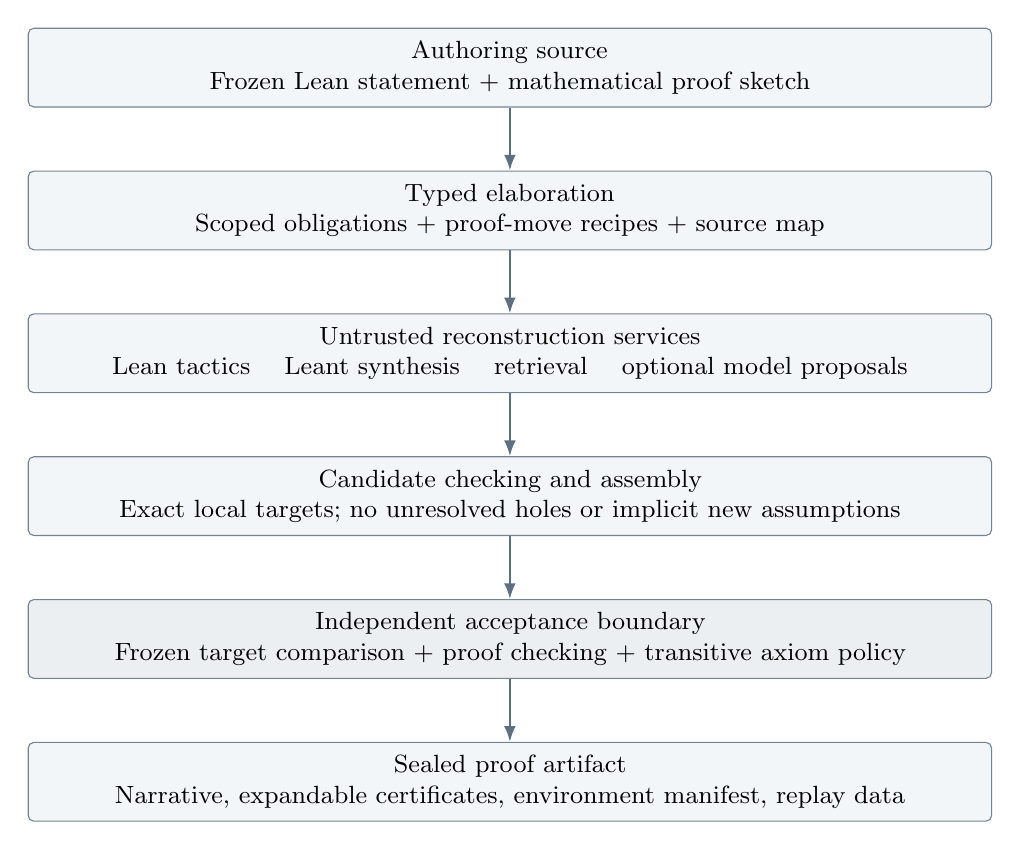
\begin{tikzpicture}[
  box/.style={draw=ink!60,rounded corners=2pt,fill=soft,align=center,text width=12cm,minimum height=10mm,font=\small},
  flow/.style={-{Latex[length=2mm]},thick,draw=ink!70},
  note/.style={font=\footnotesize,align=center,text=ink}
]
\node[box] (source) {Authoring source\\Frozen Lean statement + mathematical proof sketch};
\node[box,below=8mm of source] (graph) {Typed elaboration\\Scoped obligations + proof-move recipes + source map};
\node[box,below=8mm of graph] (search) {Untrusted reconstruction services\\Lean tactics \quad Leant synthesis \quad retrieval \quad optional model proposals};
\node[box,below=8mm of search] (assembly) {Candidate checking and assembly\\Exact local targets; no unresolved holes or implicit new assumptions};
\node[box,below=8mm of assembly,fill=ink!8] (validate) {Independent acceptance boundary\\Frozen target comparison + proof checking + transitive axiom policy};
\node[box,below=8mm of validate] (artifact) {Sealed proof artifact\\Narrative, expandable certificates, environment manifest, replay data};
\draw[flow] (source)--(graph);
\draw[flow] (graph)--(search);
\draw[flow] (search)--(assembly);
\draw[flow] (assembly)--(validate);
\draw[flow] (validate)--(artifact);
\end{tikzpicture}
\caption{Proposed architecture. Failure at any checking boundary leaves the proof unsealed.}
\label{fig:architecture}
\end{figure}

\subsection{Stage one: a minimal useful vertical slice}
Keep theorem statements in Lean. Implement only local assertions, sufficiency, calculations, named reasons, and a restricted \code{routine} service. Use the ordinary Lean context as the source of truth. Provide a clear inspection panel showing each generated obligation and its result.

The acceptance criterion is modest but concrete: several selected examples should elaborate without changing their exact statements, export ordinary Lean proofs, and reject deliberately broken versions. This stage should not support unrestricted English, automatic theorem-statement repair, or an opaque ``prove anything'' command.

\subsection{Stage two: mathematical bridge libraries}
Add a finite-sum reindexing move and a monotonicity move with explicit domains. These are directly motivated by the inspected binomial and Lambert proofs. Their side conditions are manageable, their mathematical intent is recognizable, and their failures can be explained in familiar terms.

At this stage, measure whether the authoring gain survives when bridge implementation and maintenance costs are counted. A bridge used once may be an over-engineered tactic. A bridge used in dozens of related arguments may be the real source of compression.

\subsection{Stage three: bounded synthesis and retrieval}
Integrate Leant through a narrow adapter that records the original goal and candidate origin. Initially use it only for structural composition of already selected facts. Add theorem retrieval as a suggestion service whose results become resolved, typed dependencies after verification.

The adapter needs tests for scope, universes, implicit binders, dependent opaque formulas, and changed provider inventories. It must preserve negative-result qualifications rather than flatten them into a boolean success/failure protocol. Retrieval should distinguish a theorem being developed from permissible prerequisite theorems.

\subsection{Stage four: sealed artifacts and controlled repair}
Introduce the frozen statement manifest, an export/replay path, dependency-aware cache invalidation, and a strict axiom policy. Add a hardened validation mode before enabling unreviewed model-generated code. On library upgrades, report failures at proof-move boundaries and propose local repairs without changing the approved statement.

A repair tool may suggest a new lemma, a more explicit domain, or a different proof recipe. It should show whether the change is only a proof edit or an actual change of theorem. This distinction is more important than presenting all upgrades as effortless automatic success.

\subsection{Stage five: richer mathematical notation}
Only after the earlier boundaries are reliable should the system support broader natural notation, controlled anaphora, or free-form drafting assistance. Every new notation form must expose its elaborated meaning. A fallback to ordinary Lean should remain available for difficult steps and unusual definitions.

The long-term product is therefore a mixed language: concise mathematical structure where it helps, existing Lean where it is already ideal, and explicit proof obligations wherever automation cannot safely fill the gap. Uniform surface appearance is less important than reliable meaning.

\section{How to evaluate the proposal without fooling ourselves}
\label{sec:evaluation}
A convincing evaluation must demonstrate more than a few attractive rewritten examples. The examples in this article identify design requirements; they do not measure the proposed language's effectiveness.

\subsection{Compare against strong Lean baselines}
Use at least three authoring conditions: the original repository proof, an expert-refactored Lean proof using appropriate existing abstractions and automation, and a \Motive\ proof using the same mathematical library. An optional model-assisted condition should be reported separately. Otherwise the experiment may attribute the effect of stronger automation or better library lemmas to the new language.

All conditions must prove the same elaborated proposition under the same hypotheses and permitted axioms. A prettier statement that specializes a ring to the reals, assumes a missing denominator condition, or changes an existential's scope is not a compressed proof of the original theorem.

The set should include negative controls such as the already-short normalized polynomial theorem. A language that makes those proofs longer can still be useful overall, but its evaluation must show where the tradeoff occurs.

\subsection{Prevent theorem leakage}
When a target theorem is selected for a benchmark, remove it and any impermissible downstream facts from the search environment. Searching an environment that already contains the original theorem can turn ``proof synthesis'' into a lookup. Removing only its public name is insufficient if an alias or equivalent downstream theorem remains available.

Train or tune domain packages on one part of the development and evaluate on held-out files or families of arguments. Nearby lemmas often share exactly the bridge that is being tested; a random split of almost-identical theorem statements can exaggerate generality. The permitted dependency graph should be part of the benchmark artifact.

\subsection{Measure authorship, not only displayed length}
Useful metrics include the number of authored tokens, number of explicit mathematical choices, amount of manually supplied bridge code, and time spent repairing failed obligations. Record the total certificate size and checking time separately; a short source can expand into a large proof.

One possible accounting model is
\begin{equation}
C_{\mathrm{author}}(N)=C_{\mathrm{package}}+
\sum_{i=1}^{N}\bigl(C_{\mathrm{sketch},i}+C_{\mathrm{repair},i}\bigr),
\label{eq:cost}
\end{equation}
where $C_{\mathrm{package}}$ charges the one-time work of building shared bridges. The units must be stated---tokens, editing time, or reviewed lines---rather than combining incomparable quantities. Report both the raw cost and amortized cost per proof. Hiding a large one-off bridge under a one-word command does not establish an improvement.

For the backend, record success rate, resource limits, median and tail latency, number of candidate checks, and certificate replay success. Distinguish interactive response from cold builds and from search-free replay. Resource exhaustion is a result to report, not a reason to exclude a difficult example from the denominator.

\subsection{Measure explanation and maintenance}
Human evaluation should ask readers to identify the proof's central idea, recover a missing intermediate argument, and diagnose a deliberately removed hypothesis. These tasks test whether the compressed narrative communicates mathematics, rather than whether it merely looks natural. Blind comparisons and consistent mathematical background are preferable to asking participants which syntax they like.

Maintenance tests should include harmless renamings, changed normal forms, reordered local hypotheses, and library upgrades that preserve theorem meanings. More severe tests should change an actual assumption or definition and verify that stale certificates are rejected. A fast cache that accepts an old proof in a semantically changed environment is a failure, not a performance win.

\subsection{A hypothesis to test, not a numerical promise}
The prediction is that the largest gains will occur in proofs with a stable mathematical skeleton and repeated representation bridges: finite sums, coefficient manipulations, order arguments, and applications of general transform theorems. Smaller gains are expected for proofs already expressed by a well-chosen library lemma. Problems whose main obstacle is discovering a new invariant or theorem are unlikely to become easy merely because the proof syntax is friendlier.

These are prospective expectations. This article does not provide measured compression ratios, latency reductions, or usability scores. Appendix~\ref{app:tests} specifies rejection tests that should accompany any future positive benchmark.

\section{Risks, tradeoffs, and a concrete recommendation}
\label{sec:conclusion}
There are several ways this proposal could fail. Automatic reconstruction may be too expensive for interactive use. Mathematical aliases may become another library-maintenance burden. A compressed proof may leave readers unable to tell which assumptions matter. A highly permissive frontend may prove a statement different from the one the author intended. A rigid frontend may simply replace one kind of verbosity with another.

The architecture addresses these risks by keeping proof moves local, reconstruction bounded, interpretations explicit, and certificates expandable. It does not make them disappear. In particular, determining the best level of narrative detail requires author control and empirical study. A useful tool should make it easy to add one illuminating intermediate fact even when automation could omit it.

The recommended first experiment is therefore not a general natural-language theorem prover. It is a small Lean proof-language extension with three capabilities: structured mathematical calculations, contract-based finite reindexing and monotonicity, and Leant-assisted composition of known facts. These capabilities directly target the source patterns reviewed here. They can be implemented and tested without inventing a new foundation or pretending that structural synthesis understands all the mathematical content of opaque propositions.

The proposed language's governing principle can be stated compactly:
\begin{designbox}
\textbf{Keep the mathematical decision. Generate its consequences. Check every consequence. Preserve the exact statement.}
\end{designbox}
This changes the role of a formal proof author. Instead of repeatedly programming the library's representation conventions, the author supplies a mathematical argument whose omitted details have explicit reconstruction contracts. The details still exist, but their natural home is the expandable certificate rather than the primary narrative.

\clearpage
\appendix
\section{An illustrative grammar and move interface}
\label{app:grammar}
The following grammar is a design sketch, not a parser specification or a supported syntax of Lean or Leant. It deliberately leaves term and proposition syntax to the host language.
\par\noindent\begin{minipage}{\linewidth}
\begin{lstlisting}[caption={A small possible controlled proof grammar.}]
proof       ::= "proof" header block "end"
block       ::= statement*
statement   ::= "let" name ":=" term
              | "have" name? ":" proposition justification
              | "suffices" proposition justification
              | "choose" name ":=" term
              | "obtain" binder "with" proposition "from" term
              | "calculate" calculation
              | "split" proposition case-blocks
              | "induct" name ("generalizing" names)? case-blocks
              | "conclude" proposition? justification
justification ::= "from" names ("by" reasons)?
                | "by" reasons
reasons     ::= named-rule ("using" terms)?
              | "reindex" binder ":=" term ("inverse" term)?
              | "monotonicity" ("of" term)? ("on" term)?
              | "algebra" | "arithmetic" | "routine"
\end{lstlisting}
\end{minipage}\par
Surface commands such as \code{multiply} and \code{divide_by} can be registered proof moves rather than core grammar primitives. Every registered move must have a stable typed interface and must expand into the same obligation machinery. Extensibility should not create a second, unchecked route to acceptance.

A conceptual service interface can be written as follows. The record names do not describe an existing Leant API.
\par\noindent\begin{minipage}{\linewidth}
\begin{lstlisting}[caption={Proposed logical contents of a reconstruction request and response.}]
Request = {
  environmentRevision,
  scopeId,
  dependentTelescope,
  exactTarget,
  approvedFacts,
  selectedMoveAndParameters,
  axiomPolicy,
  resourceBudget,
  originId
}

Candidate = {
  originId,
  proofTermOrValidatedExport,
  resolvedDeclarations,
  generatedSubgoalCertificates,
  producerDiagnostics
}

accept(request, candidate):
  validate the export representation
  require matching origin and compatible exact environment
  check candidate at request.exactTarget in its full telescope
  audit transitive axioms against request.axiomPolicy
  return a checked certificate; otherwise reject
\end{lstlisting}
\end{minipage}\par
Origin identifiers prevent accidental cross-association; they do not prove correctness. The type check remains authoritative. Likewise, a candidate's self-reported list of declarations or axioms is only diagnostic until independently recomputed or validated.

\clearpage
\section{An obligation ledger for one reindexing step}
\label{app:ledger}
For the move in Section~\ref{sec:worked}, a source-linked ledger could contain the following entries. ``Arithmetic'' and ``transport'' here name proposed services, not completed runs.
\begin{longtable}{@{}p{.09\textwidth}p{.57\textwidth}p{.27\textwidth}@{}}
\toprule
Node & Exact mathematical purpose & Intended discharge\\
\midrule
\endfirsthead
\toprule Node & Exact mathematical purpose & Intended discharge\\\midrule
\endhead
B1 & From $\neg(n<j)$, derive $j\leq n$. & Natural-number order\\
B2 & With $m=n-j$, derive $n=j+m$. & Arithmetic using B1\\
B3 & Show $i\leq m\Rightarrow j\leq j+i\leq n$. & Arithmetic using B2\\
B4 & Show $j\leq k\leq n\Rightarrow k-j\leq m$. & Arithmetic using B2\\
B5 & Prove the two inverse laws for $i\mapsto j+i$. & Arithmetic with bounds\\
B6 & Rewrite $n-(j+i)$ as $m-i$. & Natural subtraction theorem\\
B7 & Instantiate the binomial multiplication identity. & Resolved named theorem\\
B8 & Transport B7 from natural coefficients to $\Z$. & Homomorphism certificate\\
B9 & Establish summand equality using B6--B8. & Ring normalization\\
B10 & Assemble the finite-sum reindexing and factorization. & Reindexing and sum lemmas\\
\bottomrule
\end{longtable}
The ledger is intentionally more explicit than the authored sketch. Its purpose is not to force the author to read all ten nodes each time. Its purpose is to make the compressed line expandable, diagnosable, and independently checkable. A real implementation may fuse several nodes or use a different internal proof while preserving the same mathematical move contract.

\clearpage
\section{Conformance and adversarial tests}
\label{app:tests}
The following tests are proposed acceptance criteria. They have not been executed against a Motive implementation.
\begin{longtable}{@{}p{.06\textwidth}p{.39\textwidth}p{.48\textwidth}@{}}
\toprule
 & Test input or mutation & Required behavior\\
\midrule
\endfirsthead
\toprule & Test input or mutation & Required behavior\\\midrule
\endhead
1 & Normalize at $q=1,n=1$ and claim mass one without a denominator hypothesis. & Reject that claim; exhibit the unmet nonzero condition.\\
2 & Normalize at $n=0$ with arbitrary $q$. & Permit the proof without inventing a condition $q\ne0$.\\
3 & Replace $j\leq n$ by no assumption in $j+(n-j)=n$. & Do not apply integer-style subtraction; leave or refute the obligation.\\
4 & Float the witness $m+1$ outside the scope of $m$. & Reject the escaping local variable.\\
5 & Use a branch-local hypothesis in the other case. & Reject scope mismatch, including through a cache.\\
6 & Use restricted monotonicity without one membership proof. & Generate the missing domain obligation, not a global monotonicity assertion.\\
7 & Multiply a strict inequality by a merely nonnegative factor. & Require positivity or a different argument covering the zero case.\\
8 & Treat opaque $0=0$ as an unprovable atom in a search fragment. & Never report that the original Lean equality is false.\\
9 & Exhaust a finite search budget. & Report \code{UnknownBudget}, not a proof of noninhabitation.\\
10 & Use classical reasoning under a constructive policy. & Reject unapproved dependencies or require an explicit policy change.\\
11 & Hide \code{sorryAx} or a computation axiom in a dependency. & Reject under the strict allowlist even when the top-level script has no \code{sorry}.\\
12 & Change a type-class instance or referenced definition while retaining the printed statement. & Invalidate affected certificates and compare the exact new target.\\
13 & Supply a correct proof term with a forged candidate origin. & Reject the association; do not transfer evidence by text similarity.\\
14 & Solve a benchmark by a hidden alias of the target theorem. & Mark the run invalid under its dependency policy.\\
15 & Claim limit interchange using only pointwise convergence. & Require the selected interchange theorem's additional hypotheses.\\
16 & Keep the reason ``by lemma L'' after a solver uses an unrelated route. & Do not retain that reason as verified recipe provenance; request an explanation update.\\
\bottomrule
\end{longtable}

\clearpage
\section{Source ledger and reproducibility boundaries}
\label{app:sources}
\subsection*{Pinned repository snapshots}
\noindent\textbf{ProveIt}\par
\noindent\Pcommit\par
\noindent\textbf{Leant}\par
\noindent\Lcommit

\noindent These are the repository revisions resolved during the review. Their identification pins the observations, not the entire external mathematical library or build toolchain. No repository build or Lean proof replay was performed for this article.

\begin{longtable}{@{}p{.60\textwidth}p{.33\textwidth}@{}}
\toprule
Inspected source & Scope used in this article\\
\midrule
\endfirsthead
\toprule Inspected source & Scope used in this article\\\midrule
\endhead
\pfile{BinomialInversion.lean} & Entire file; orthogonality, transform application, module/ring presentation.\\
\pfile{LambertWElementaryBounds.lean} & Entire file; tangent inequality, branch conditions, elementary chain.\\
\pfile{GeometricRichardson.lean} & Lines 1--260; raw polynomial facts and initial normalization results.\\
\lfile{README.md} & Introductory and selected synthesis/proof-mode material, including lines 330--610 at the pinned revision.\\
\lfile{docs/synth-internals.md} & Lines 1--230; architecture, semantic origin, candidate/evidence associations.\\
\lfile{src/Leant/Synth/Fragment.hs} & Lines 1--220; fragment representation and its stated translation boundaries.\\
\bottomrule
\end{longtable}
The source files named above are the evidential basis for repository-specific observations. Statements about the wider Lean ecosystem are supported by the primary references below. The bibliography is selective, not a survey claiming coverage of every declarative proof language or recent autoformalization system.

\subsection*{What is reproducible from this package}
The accompanying \code{motive.tex} is self-contained apart from standard TeX packages. The PDF can be rebuilt by running \code{pdflatex} twice. The package also includes a machine-readable source manifest and a README. It contains no Motive compiler, no purportedly verified generated Lean proof, and no fabricated benchmark data. Its mathematical derivations and design arguments can be reviewed directly; implementing and experimentally validating the proposed language remains a separate engineering project.

\clearpage
\phantomsection
\addcontentsline{toc}{section}{References}
\begin{thebibliography}{99}
\small\raggedright
\bibitem{proveit}
Vladimir Reshetnikov and contributors.
\emph{ProveIt}. Source repository, revision
\texttt{24ce8bd743eaab64a91ce90725ea00f498d319d2}.
Selected files and inspected ranges are given in Appendix~\ref{app:sources}.
\url{https://github.com/VladimirReshetnikov/ProveIt/tree/24ce8bd743eaab64a91ce90725ea00f498d319d2}.

\bibitem{leant-readme}
Leant contributors.
\emph{Leant---a Djex-based synthesis REPL for Lean 4}. README, revision
\texttt{c36adf114035fb2fba6c276b63944cc613b31668}.
\url{https://github.com/VladimirReshetnikov/Leant/blob/c36adf114035fb2fba6c276b63944cc613b31668/README.md}.

\bibitem{leant-internals}
Leant contributors.
\emph{\texttt{:synth} internals}. Revision as in reference~\cite{leant-readme}.
\url{https://github.com/VladimirReshetnikov/Leant/blob/c36adf114035fb2fba6c276b63944cc613b31668/docs/synth-internals.md}.

\bibitem{leant-fragment}
Leant contributors.
\emph{\texttt{Leant.Synth.Fragment}}. Source code, revision as in reference~\cite{leant-readme}.
\url{https://github.com/VladimirReshetnikov/Leant/blob/c36adf114035fb2fba6c276b63944cc613b31668/src/Leant/Synth/Fragment.hs}.

\bibitem{lean4}
Leonardo de Moura and Sebastian Ullrich.
\emph{The Lean 4 Theorem Prover and Programming Language (System Description)}.
CADE, 2021.
\url{https://lean-lang.org/papers/lean4.pdf}.

\bibitem{lean-elab}
Lean development team.
\emph{The Lean Language Reference: Elaboration and Compilation}.
Online reference, consulted September 5, 2026.
\url{https://lean-lang.org/doc/reference/latest/Elaboration-and-Compilation/}.

\bibitem{lean-trust}
Lean development team.
\emph{The Lean Language Reference: Validating a Lean Proof}.
Online reference, consulted September 5, 2026. Includes version-qualified discussion of native evaluation and stronger validation workflows.
\url{https://lean-lang.org/doc/reference/latest/ValidatingProofs/}.

\bibitem{isar}
Isabelle project.
\emph{Isar---Intelligible semi-automated reasoning}.
Project overview and primary-publication index.
\url{https://isabelle.in.tum.de/Isar/}.

\bibitem{naproche}
Naproche project.
\emph{The Naproche project: Investigating Mathematical Text}.
Project overview.
\url{https://naproche-net.github.io/}.

\bibitem{verbose}
Patrick Massot and contributors.
\emph{Verbose Lean 4}. Project source and README.
\url{https://github.com/PatrickMassot/verbose-lean4}.

\bibitem{gflean}
Shashank Pathak.
\emph{GFLean: An Autoformalisation Framework for Lean via GF}.
arXiv:2404.01234, 2024.
\url{https://arxiv.org/abs/2404.01234}.

\bibitem{aesop}
Jannis Limperg and Asta Halkj{\ae}r From.
\emph{Aesop: White-Box Best-First Proof Search for Lean}.
Certified Programs and Proofs (CPP), 2023.
\url{https://doi.org/10.1145/3573105.3575671}.

\bibitem{grind}
Lean development team.
\emph{The Lean Language Reference: The \texttt{grind} tactic}.
Online reference, consulted September 5, 2026.
\url{https://lean-lang.org/doc/reference/latest/The--grind--tactic/}.

\bibitem{formalign}
Jianqiao Lu, Yingjia Wan, Yinya Huang, Jing Xiong, Zhengying Liu, and Zhijiang Guo.
\emph{FormalAlign: Automated Alignment Evaluation for Autoformalization}.
arXiv:2410.10135, 2024.
\url{https://arxiv.org/abs/2410.10135}.
\end{thebibliography}
\end{document}
